\documentclass[11pt]{article}

\usepackage{fullpage,times}%charter}
\usepackage{color}

\usepackage{tikz}
%\usetikzlibrary{arrows.meta}
\usetikzlibrary{automata}
%% macros
\newcommand{\ax}[1]{\texttt{AX}(#1)}
\newcommand{\ex}[1]{\texttt{EX}(#1)}
\newcommand{\af}[1]{\texttt{AF}(#1)}
\newcommand{\ef}[1]{\texttt{EF}(#1)}
\newcommand{\ag}[1]{\texttt{AG}(#1)}
\newcommand{\eg}[1]{\texttt{EG}(#1)}
\newcommand{\au}[2]{\texttt{A}(#1\ \texttt{U}\ #2)}
\newcommand{\eu}[2]{\texttt{E}(#1\ \texttt{U}\ #2)}
\newcommand{\sem}[1]{[\!\![#1]\!\!]}

\newcommand{\euntil}[3]{\texttt{E}(#1\ \texttt{U}^{#3}\ #2)}
\newcommand{\auntil}[3]{\texttt{A}(#1\ \texttt{U}^{#3}\ #2)}


\newcommand{\lx}[1]{\texttt{X}(#1)}
\newcommand{\lf}[1]{\texttt{F}(#1)}
\newcommand{\llg}[1]{\texttt{G}(#1)}
\newcommand{\lu}[2]{(#1\ \texttt{U}\ #2)}


\newcommand{\sol}[1]{{\color{blue}#1}}
%\newcommand{\sol}[1]{}
\begin{document}

\hrule
\smallskip

\noindent

\noindent
You can review the latex source for this assignment-file to
learn and use latex to prepare your homework submission. You will see
the use of macros (to write uniformly formatted text), different
text-styles (emphasized, bold-font), different environments (figures,
enumerations).

It is not required that you use exactly this latex source to prepare
your submission. 
\smallskip
\hrule


\begin{center}
{\Large\bf Homework 5 (CTL/LTL/PCTL): ComS/CprE/SE 412, ComS 512}

\medskip

Due-date: May 3 at 11:59PM.

\medskip


\end{center}

\noindent
\textbf{
Submit online on Canvas two files: the source file in latex format and
the pdf file generated from latex. Name your files:
$\langle\mbox{your-net-id}\rangle$-hw5.$\langle\mbox{tex/pdf}\rangle$.
}

\hrule
\noindent
\smallskip

\emph{ Homework must be individual's original work. Collaborations and
  discussions of any form with any students or other faculty members
  or soliciting solutions on online forums are not allowed. Please
  review the academic dishonesty policy on our syllabus. If you have
  any questions/doubts/concerns, post your questions/doubts/concerns
  on Piazza and ask TA/Instructor.}

\smallskip
\hrule

\begin{enumerate}

\item 
Consider the following DTMC

\begin{center}
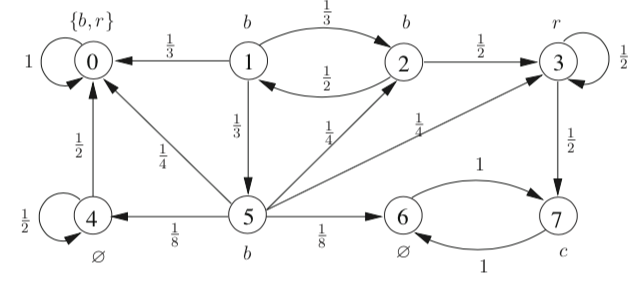
\includegraphics[scale=0.5]{images/dtmc-hw-katoen.png}
\end{center}
The states are numbered. The propositions of interest are $b$, $c$ and
$r$. Determine the set of states which satisfy the PCTL formula
$\mathtt{P}_{\geq \frac{17}{19}}\lu{(b\lor\neg r)}{c}$. Show the steps of your computation
(either using linear equation based method or by matrix-vector multiplications).
\hfill(8pts)

\textbf{Answer}:


The linear equations can be formed as follows- 

\[x_0=0\]
\[x_1=\frac{1}{3}x_2 + \frac{1}{3}x_0 + \frac{1}{3}x_5\]
\[x_2 = \frac{1}{2}x_3 + \frac{1}{2}x_1\]
\[x_3=0\]
\[x_4=\frac{1}{2}x_4 + \frac{1}{2}x_0\]
\[x_5 = \frac{1}{4}x_0 + \frac{1}{4}x_2 + \frac{1}{4}x_3 + \frac{1}{8}x_4 + \frac{1}{8}x_6 \]
\[x_6 = x_7\]
\[x_7=1\]

In the next line, we can simply as follows- 

\[x_0=0\]
\[x_1=\frac{1}{3}x_2 + \frac{1}{3}x_5\]
\[x_2 = \frac{1}{2}x_1\]
\[x_3=0\]
\[x_4=0\]
\[x_5 =  \frac{1}{4}x_2 + \frac{1}{8} \]
\[x_6 = 1\]
\[x_7=1\]

After this, we can write the above equations as follows- 

\[x_0=0\]
\[x_1=\frac{1}{6}x_1 + \frac{1}{12} x_2 + \frac{1}{24}\]
\[x_2 = \frac{1}{2}x_1\]
\[x_3=0\]
\[x_4=0\]
\[x_5 =  \frac{1}{4}x_2 + \frac{1}{8} \]
\[x_6 = 1\]
\[x_7=1\]

By solving these equations, we get, \(x_0=0, x_1=\frac{1}{18}, 
x_2=\frac{1}{36}, x_3=0, x_4=0, x_5=\frac{1}{136}+\frac{1}{8}, x_6=1, x_7=1\). Therefore, the set of states satisfying $\mathtt{P}_{\geq \frac{17}{19}}\lu{(b\lor\neg r)}{c} = \{s_6, s_7\}$



\item 
Prove or disprove the following:
\begin{enumerate}
\item 
If a state in a DTMC does not satisfy $\mathtt{P}_{\geq 1}(\lf{\neg q})$ then 
it must satisfy $\eg{q}$ in the same system.

\textbf{Answer}: 

If a state in a DTMC does not satisfy $\mathtt{P}_{\geq 1}(\lf{\neg q})$, which means a state in DTMC satisfies $\llg{q}$ with some probability greater than 0. Furthermore, satisfying a formula with a probability greater than 0 implies path quantifier $E$. From this, we can immediately say that there exists at least one path from s that satisfies $\eg{q}$.  

$\mathtt{P}_{\geq 1}(\lf{\neg q})$ 
$\leftrightarrow \mathtt{P}_{>0}(\neg (\lf{\neg q}))$
$\leftrightarrow \mathtt{P}_{>0}(\llg{ q})$
$\leftrightarrow (\eg{q})$

Therefore, this statement is satisfied.

\item 
If a state in a DTMC satisfies $\mathtt{P}_{\leq 0}(\llg{\neg q})$ then it must satisfy $\ag{q}$ in the same system.

\textbf{Answer}: 
$s \models \mathtt{P}_{\leq 0}(\llg{\neg q})$

$s \models \mathtt{P}_{\geq 1-0}(\neg (\llg{\neg q}))$

$s \models \mathtt{P}_{\geq}((\lf{ q}))$

This implies that the probability of satisfying $\lf{ q}$ is equal to 1, therefore, the system does not satisfy $\ag{q}$. 

\end{enumerate}
\hfill(6pts)

\item 
Consider a Kripke structure $(S, T, L)$ such that
\begin{itemize}
\item  $S = \{s_1, s_2, s_3, s_4, s_5\}$
\item $T = \{(s_1, s_3), (s_1, s_4), (s_2, s_4), (s_3, s_4), (s_4, s_2), (s_4, s_3), (s_4, s_5), (s_5, s_4), (s_5, s_5)\}$
 where $(s, s') \in T$
implies $s$ has a transition to $s'$;
\item $L(s_1) = \{a\}, L(s_2) = \{c\}, L(s_3) = \{b, c\}, L(s_4) = \{a, b, c\}$
\end{itemize}
Decide for each of the LTL formulas $\varphi_i$ below whether $s_1 \models \varphi_i$. If $s_1 \not\models \varphi_i$, 
present a path $\pi$ such that $\pi[0] = s_1$ and $\pi \not\models \varphi_i$.
\begin{enumerate}
\item $\varphi_1 = \lf{\llg{c}}$

\textbf{Answer}: The path not satisfying $\varphi_1 = \lf{\llg{c}}$ is \(\pi = s_1,s_4,s_5,s_5,s_5,...\). 

\item $\varphi_2 = \llg{\lf{c}}$

\textbf{Answer}: The path not satisfying \(\pi = s_1,s_3,s_4,s_5,s_5,s_5,...\)
\item $\varphi_3 = \lx{\neg c} \Rightarrow \lx{\lx{c}}$
%(d) φ4 = a U G(b ∨ c

\textbf{Answer}: \(\varphi_3 = \lx{\neg c} \Rightarrow \lx{\lx{c}} \leftrightarrow \neg \lx{\neg c} \lor \lx{\lx{c}} \leftrightarrow \lx{c} \lor \lx{\lx{c}} \). 
All paths starting from $s_1$ satisfies $\lx{c}$, so the system 
satisfies this formula. 
\end{enumerate}
\hfill(6pts)
\end{enumerate}


\end{document}

